% Created 2020-07-29 Wed 18:43
% Intended LaTeX compiler: pdflatex
\documentclass[a4paper]{article}
\usepackage[utf8]{inputenc}
\usepackage[T1]{fontenc}
\usepackage{graphicx}
\usepackage{grffile}
\usepackage{longtable}
\usepackage{wrapfig}
\usepackage{rotating}
\usepackage[normalem]{ulem}
\usepackage{amsmath}
\usepackage{textcomp}
\usepackage{amssymb}
\usepackage{capt-of}
\usepackage{hyperref}
\author{Tigany Zarrouk}
\date{\today}
\title{Multi-scale investigation of dislocation mediated carbon migration in iron}
\hypersetup{
 pdfauthor={Tigany Zarrouk},
 pdftitle={Multi-scale investigation of dislocation mediated carbon migration in iron},
 pdfkeywords={},
 pdfsubject={},
 pdfcreator={Emacs 26.3 (Org mode 9.1.9)}, 
 pdflang={English}}
\begin{document}

\maketitle
\tableofcontents

\begin{abstract}

We investigate the validity of a dislocation-assisted carbon migration
mechanism underpinning the formation of dark etching regions in
bearing steels undergoing high-cycle fatigue through use of a
multi-scale approach: from quantum mechanics,
to stochastic simulations. We start from tight binding simulations of
$1/3\langle 111 \rangle$ screw dislocations to obtain the 2-d Peierls
potential and Fe-C binding energies. These become ingredients for a line-tension
model of the $1/3\langle 111 \rangle$ screw dislocation to obtain the kink-pair formation
energy as a function of stress and carbon concentration. Finally,
3-d kinetic Monte-Carlo simulations of dislocations in an environment
of carbon are used to ascertain which temperature and stress regimes
dislocation-assisted carbon migration is a valid mechanism. 

\end{abstract}


\section{Introduction}
\label{sec:org1fae4f5}

\begin{itemize}
\item Outline of the literature review 
\begin{enumerate}
\item Origin of DER formation through high-cycle fatigue
\item What is the DER region and what phases is it composed of?
\item What are the current mechanisms which explain this?
\begin{enumerate}
\item Why are they insufficient?
\end{enumerate}
\item Ouline of the work considering Fe-C dislocation modelling
\end{enumerate}
\end{itemize}


Martensitic steels are frequently used in bearings due to their
resilience to service conditions, such as high rotational speeds and
contact pressures. However, under cyclic loading exceeding a given
contact stress (the elastic shakedown limit), the microstructure of
the steel can decay, signalling the onset of rolling cycle fatigue
(RCF), enhancing the risk of failure from subsurface crack
initiation. This microstructural decay corresponds to Dark Etching
Regions (DERs) as seen in optical images, where the darkness of the images
is due to the higher reactivity of the phases which compose the DER
region to the etchant, exacerbated by the roughness of the DER
region, with more grains per unit
area scattering light.

Further development of the DER occurs with more stress cycles (of
which development is hastened with a higher contact
pressure). Matured DER regions have additional features, such as
white etching bands (WEBs), which occur at specific angles (\(30\deg
  / 80\deg\), for low angle / high angle WEBs respectively).

DERs are found in the subsurface of the material, due to the maximum
deviatoric stress being found in the subsurface from the Hertzian
stress distribution exhibited by bearing contact. 


These DER regions are composed of multiple different phases. They are
generally defined to be mixtures of ferritic features within a
residual martensitic matrix initially, but there are other phases
which appear upon the further degredation of martensite during RCF. 

There are: ferrite microbands which are generally grouped together;
elongated ferrite, which may be composed by multiple ferrite
microbands joining together---these have also been seen to form WEBs
along with ferrite microbands; residual carbides, in which ferrite
(microbands and elongated) can form inside of, causing it to
dissolve; lenticular carbides, which are formed on the side and
parallel to WEBs, and are observed in conjunction with the formation
of WEBs.

It is thought that the formation of lenticular carbides is related
to the dissolution of residual cementite and tempered carbides,
increasing the carbon content within the the ferrite
microbands/nanocrystalline ferrite (DER) and reducing solubility of
the carbon within WEBs. Residual cementite does not need to by fully
dissolved for the formation of lenticular carbides. 

Fu \emph{et al.} have claimed that carbon is redistributed into higher
carbon concetrated regions such as cementite and other transition
carbides. 



\begin{itemize}
\item Elucidate on the measurements pertaining to the migration of
carbon
\end{itemize}


Many authors have proposed that carbon plays a crucial role in the
formation of the DER regions. 

Voskamp suggests that cyclic stresses generate a local rise in
temperature, which promotes diffusion of atomic carbon trapped in
the martensitic matrix. With diffusion of carbon, dislocations
become unpinned, enabling potential slip systems to activate. The
unpinned dislocations cause deformation. 

Polonsky and Keer propose that the redistribution of the carbon
solutes cause the formation of ferrite microbands by 
cyclic-plastic strain induced softening. Carbon redistribution
is caused by the release of carbon trapped by dislocations with the
application of stress. 

Due to the high dislocation density of martensite, all dissolved
carbon is segregated to dislocations---which also pin the
dislocations. With applied stress, the dislocations become unpinned
and mobile. Dislocations multiply/annihilate; with annihilation,
carbon becomes in ordinary solution, which is available to
diffuse. This diffusion causes the formation of ferritic
microbands. The process of annihilation needs to be understood. 

Hedman/Slycke propose that the degradation of the DER can by
described by the growth of carbides, where the carbide sized are
described by Ostwald ripening, and carbon diffuses both thermally
and mechanically by dislocation glide. 

Slycke proposes a creep deformation based mechanism which is
controlled by vacancies produced by the climb of dislocations. 

Fu \emph{et al.} propose that the fundamental mechanism to DER formation
is carbon migration under RCF driven by gliding dislocations. Strain
generated by pulsating stresses allow dislocations to escape their
carbon rich environment. The dislocations, now free, re-attract
carbon, allowing the Cottrell atmosphere to reform, subsequently
pinning the dislocation. This creates a net carbon flux. But, if
carbides were to form in martensite, they should follow the
Bagaryatskii/Isaichev orientation relationship. The cementite formed
within the DER region, has an irregular shape, which must be due to
te incomplete dissolution of residual cementite. 

Smelova proposes that the formation of elongated ferrite are the
result of recrystallisation processes. 

\subsection{Mechanisms}
\label{sec:orge7398a2}

There are many proposed mechanisms for DER formation.

Bush proposes that DER formation is governed by an
exchange of material between the carbides and the matrix, which is
evidenced by the formation of intrusions/extrusions within the
microstructure. 

Swahn proposes that the transformation mechanisms which lead to the
formation of new features in DER are due to the redistribution of
carbon present in the initial microstructure, which in solution in
the martensite, and due to the dissolution of carbides. 

They further detail that initially, stress induced carbon diffusion
leads to the diffusion of carbon from the martensitic lattice to
the various defects in the material (mainly dislocations). 
As plastic deformation accumulates, the movement of dislocations
creates carbon rich grain boundary-type interfaces. 

It is not certain what role and timescale the dissolution of
carbides occurs on. 

High operating temperatures are known to accelerate DER formation. 

In early stage DER formation, there is a high density of ferrite
microbands. Later, regions of homogeneous nanocrystalline ferrite
(heavily deformed ferrite) are formed in a cell-like structure.







\section{Computational Method}
\label{sec:orgcdfc6ac}

\begin{itemize}
\item Use tight-binding model of Paxton and Elsaetter \cite{Paxton2013}.
\item Generate dislocations using anisotropic elasticity theory.
\item Create clusters of dislocations in both easy and hard core
configurations.
\item Place carbon in octahedral sites around the core
\item Calculate corrections (ZPE etc)
\end{itemize}


\section{Results}
\label{sec:orgf76a3b1}



\subsection{Peierls Potential}
\label{sec:orgd9a2cc3}

To determine the Peierls potential, we followed the procedure detailed in Itakura
\cite{Itakura2012}. Quadrupolar arrays of dislocations were constructed by placing dislocations of
antiparallel \(1/2\langle 111\rangle\) Burgers vectors in an "S" arrangement \cite{Clouet2012}, with
initial displacements determined by the anisotropic elasticity solutions. These displacements
were modified to be periodic, thereby removing artificial stacking faults which would appear
between periodic images after the introduction of the dipole. This was achieved by the subraction
of a linear error term from the superposition of displacement fields arising from the
dislocations in the simulation cell and its periodic images \cite{vasilybulatov2006}. To accomodate
for the internal stress upon introduction of the dislocation dipole into a simulation cell, an
elastic strain was imposed on the cell, resulting in an extra tilt component being added to the
cell vectors \cite{Clouet2012,vasilybulatov2006}. Simulation cells were constructed with different
initial core positions, which were sampled from the triangular region "EHS" (easy, hard and
split) core positions, as detailed in \ref{fig:peierlspot}. To fix the dislocation positions during
relaxation, the three atoms surrounding the easy core, for each dislocation, were fixed during
relaxation. 

I do not agree with the calculation of the interaction energy between dislocations in
Itakura's paper. Their equation is a sum over periodic images, which leads to
a problem in the conditional convergence of the interaction energy, as shown by Bulatov
and Cai \cite{vasilybulatov2006}. The equation found in Itakura would clearly depend on
the truncation limit for the sum, which they do not specify. 

The interaction energy between the dislocation dipole and periodic images
should follow the prescription of Bulatov and Cai \cite{vasilybulatov2006}. In
isotropic elasticity, the elastic energy of a single dislocation dipole in an
infinite lattice is given by


\[ E_{\text{el}}^{\inf} = \frac{\mu b^2}{4\pi} ln( \frac{r}{r_{c}} )  \]

The contribution from periodic images to the correction is 

\[ E_{\text{img} } = E_{\text{el}} (\mathbf{a}, \mathbf{c}_i , r_c) - E_{\text{el}}^{\inf}
   (\mathbf{a}, r_c)\], 

where 

\[ E_{\text{img} = \sum_{\mathbf{R}}' E_{\text{dd}} (\mathbf{R}), \]

where \(\mathbf{R}\) is a sum over dislocation dipoles in the periodic images
exclusively. 

\[ E_{\text{dd}} (\mathbf{R}) = \frac{\mu b^2}{2\pi}
   \text{ln}\frac{|\mathbf{R}|^2}{|\mathbf{R}+\mathbf{a}|\cdot|\mathbf{R}-\mathbf{a}|}
   \]

"Ghost" dipoles are introduced to account for the conditional convergence
of the sum at \(\pm\alpha \mathbf{b}\) and \(\pm \beta\mathbf{b}\), where \(\alpha = \beta = 0.5\).  


The Peierls potential can be calculated by subtraction of the interaction energy of the
dislocations in the periodic array, from the energy of the easy core
configuration, which is the ground-state dislocation core configuration. 

\[ \Delta E_{\text{P}} = \Delta E^{\text{tbe}} - \Delta E_{\text{INT}} \]



        \begin{table}
    \begin{tabular}{c}
	     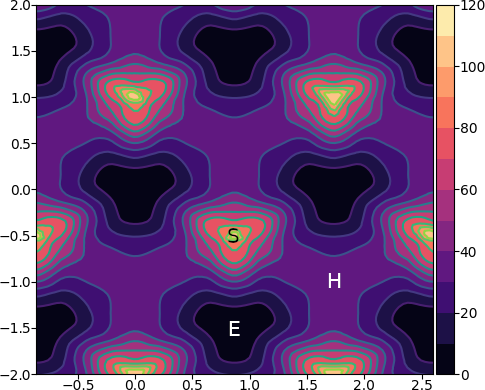
\includegraphics[width=0.8\textwidth]{../Images/itakura_dislocation_energy_landscape_2_labelled.png} \\
             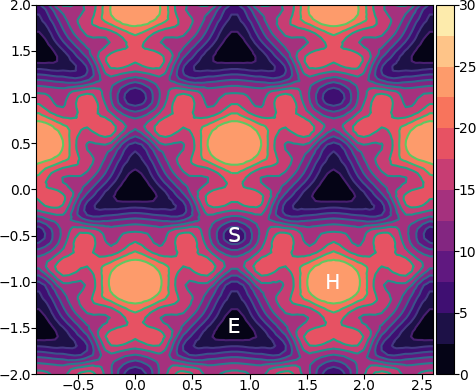
\includegraphics[width=0.8\textwidth]{../Images/tbe_dislocation_energy_landscape_pure_labelled.png}  \\
    \end{tabular}		
\caption{Comparison of 2d Peierls potentials of the $1/2\langle 111\rangle$ screw dislocation between DFT cite:Itakura2012 (top) and tight-binding (bottom). Data was interpolated using cubic splines. Energies are in $meV$, with x and y scales in units of $\sqrt{2} a_{\text{bcc}} = 2\sqrt{2/3}b$. "E", "H" and "S" correspond to easy, hard and split core positions respectively, with the latter also corresponting to atomic positions. The relative energies between the different core positions is smaller in tight-binding compared to DFT. The split core as seen in tight-binding is reminiscent of EAM potentials, where the split core energy is lower than that of the hard core. Some of this discrepancy can be attributed to the difference in simulation method: the cluster method may inhibit the relaxation of the core more than quadrupolar cells, due to finite size effects.}
	\label{fig:peierlspot}
    \end{table}



        \begin{table}
    \begin{tabular}{c}
	     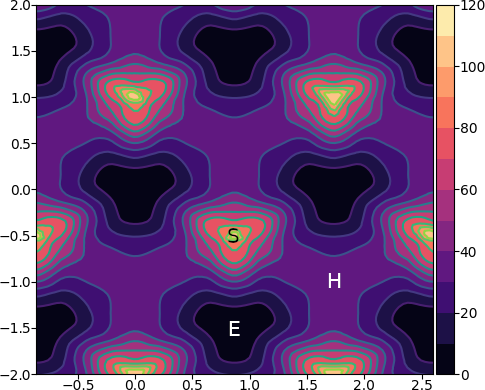
\includegraphics[width=0.8\textwidth]{../Images/itakura_dislocation_energy_landscape_2_labelled.png} \\
             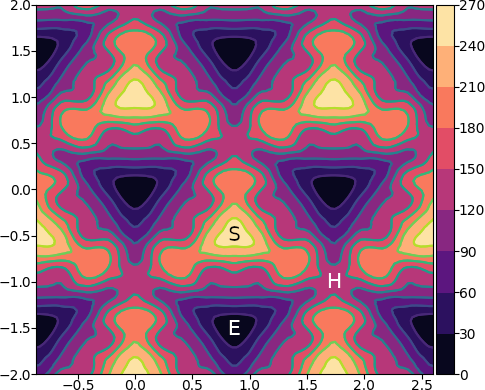
\includegraphics[width=0.8\textwidth]{../Images/tbe_dislocation_energy_landscape_2_labelled.png}  \\
    \end{tabular}		
\caption{Comparison of 2d Peierls potentials of the $1/2\langle 111\rangle$ screw dislocation between DFT cite:Itakura2012 (top) and tight-binding (bottom). Data was interpolated using cubic splines. Energies are in $meV$, with x and y scales in units of $\sqrt{2} a_{\text{bcc}} = 2\sqrt{2/3}b$. "E", "H" and "S" correspond to easy, hard and split core positions respectively, with the latter also corresponting to atomic positions. The relative energies between the different core positions is smaller in tight-binding compared to DFT. The split core as seen in tight-binding is reminiscent of EAM potentials, where the split core energy is lower than that of the hard core. Some of this discrepancy can be attributed to the difference in simulation method: the cluster method may inhibit the relaxation of the core more than quadrupolar cells, due to finite size effects.}
	\label{fig:peierlspot2}
    \end{table}


Comparison of 2d Peierls potentials of the \(1/2\langle 111 \rangle\) screw dislocation between
DFT can by found in \cite{Itakura2012}. Data was interpolated using 2d cubic splines. "E", "H"
and "S" correspond to easy, hard and split core positions respectively, with the latter also
corresponding to atomic positions. The relative energies between the different core
positions is smaller in tight-binding compared to DFT; most notably, the energies. This is
an artifact in the model, which has been validated in NEB calculations of the \(1/2\langle
	111\rangle\) screw dislocation Peierls barrier, as calculated with NEB, is roughly half that
when compared to DFT \textbf{ref Luke's Thesis}. The split core as seen in
tight-binding is reminiscent of EAM potentials, where the split core energy is lower than
that of the hard core, \emph{but first, to check that this is so, one must check that
the interaction energy between dislocations follows Bulatov and Cai}.

This may be attributed to lack of core electron	repulsion, resulting from the sd-iron tight-binding model. 

\begin{center}
\begin{tabular}{rrrrr}
Pos & \(\Delta E_{\text{INT}}\) & \(\Delta E_{\text{tbe}}\) & \(\Delta E_{\text{P}}\) & \(\Delta E_{\text{P}}^{\text{DFT}}\)\\
\hline
1 & 0 & 0 & 0 & 0\\
2 & -0.7 & 7.3 & 7.9 & 3.2\\
3 & -1.4 & 16.0 & 17.4 & 19.2\\
4 & -2.0 & 22.2 & 24.2 & 31.1\\
5 & -2.5 & 24.8 & 27.4 & 39.3\\
6 & -3.3 & 3.0 & 6.3 & 11.5\\
7 & -6.5 & 7.1 & 13.6 & 39.9\\
8 & -9.6 & 13.0 & 22.6 & 75.2\\
9 & -12.5 & 5.4 & 17.9 & 108.9\\
10 & -4.8 & 22.1 & 26.9 & 34.8\\
11 & -7.2 & 18.2 & 25.4 & 37.9\\
12 & -9.8 & 14.0 & 23.8 & 60.7\\
13 & -3.8 & 11.5 & 15.3 & 17.6\\
14 & -6.9 & 15.1 & 22.0 & 29.9\\
15 & -4.3 & 18.6 & 22.9 & 39.7\\
\end{tabular}
\end{center}

\subsection{Hard and easy core relaxations}
\label{sec:org399e230}

To determine the binding energy of carbon to dislocations, we used the
cluster method; where the simulation cells consist of a circular cluster of
atoms, split into two regions, with a single dislocation introduced into the
centre by using the anisotropic elasticity solutions. Each of the clusters
were centred on the easy or hard core positions. The cluster of atoms was
split into two regions: a central region of dynamic atoms with radius \(R_1\),
and an annulus of atoms, between \(R_1\) and \(R_2\), which were fixed to the anisotropic
elasticity solutions. 

Initially, large cells of with \(R_1 = 6\sqrt{2}a_{\text{bcc}}\), and \(R_2 =
   7\sqrt{2}a_{\text{bcc}}\) and depth of single burger's vector, were relaxed
for both the easy and hard cores, which consisted of 522 and 540 atoms
respectively. The three atoms surrounding the core were constrained, to only
relax in \(X-Y\) plane, to stop the core from moving upon relaxation. The
k-point sampling mesh for each of these cells was 1x1x24, with a charge
tolerance for self-consistency of \(1e-6\). Atoms were relaxed until the force
on each atom was less than \(1e-3\) eV/\AA{}.  

From the relaxed cells, a smaller region of 174 atoms, with \(R_1 =
   3\sqrt{2}a_{\text{bcc}}\), and \(R_2 = 4\sqrt{2}a_{\text{bcc}}\), was cut from
the dynamic regions. This smaller cell was extended to a thickness of 3b in
the Z direction. Carbon interstitials were inserted into octahedral sites
near the dislocation core, in the middle layer. Exploiting reflection and
rotational symmetry, allows us to use only 10 interstitial
sites to obtain the binding energies of carbon \(\sim 1.8\) b from the core. 

The three atoms surrounding the core in the first and third layers were again
constrained to relax only in the \(X\) and \(Y\) directions. No such constraints
were imposed on the middle layer. 

The core energy difference can be estimated by the difference
between the excess energies of the easy and hard cores in the limit
that \(\text{ln}{\frac{R}{R_0}) \rightarrow 0\). At the smallest
value, one finds that the core energy difference \(\Delta
   E_c^{\text{Easy-Hard}} = 76\) meV/b. This is in agreement with the
results of Itakura \cite{Itakura2012}, of 82 meV/b.


As found in DFT simulations by Ventelon \cite{Ventelon2015}, when a carbon was placed in the
vicinity of a relaxed easy dislocation core---in either of the two nearest, distinguishable,
octahedral sites---a spontaneous reconstruction of the dislocation core occurred: from easy to
hard. Upon reconstruction, the dislocation core moved to a neighbouring triangle, when looking along the \(\langle
   111\rangle\) direction, where the carbon found itself situated in the centre.




Plot of dislocation energy as function of cluster size. 


\begin{center}
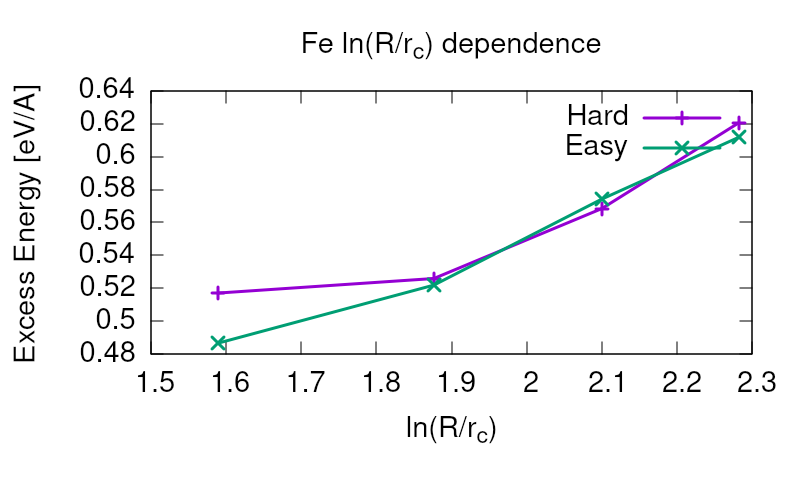
\includegraphics[width=.9\linewidth]{/home/tigany/Documents/docs/Management/Images/img_fe_size_dependence_on_log_of_core_radius.png}
\end{center}



\begin{table}	
    \begin{tabular}{c}
 	          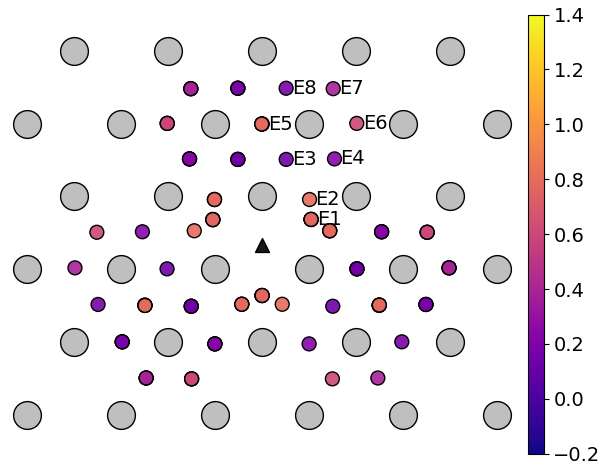
\includegraphics[width=0.85\textwidth]{../Images/easy_core_fe_C_positioning_energies.png}  \\
 	          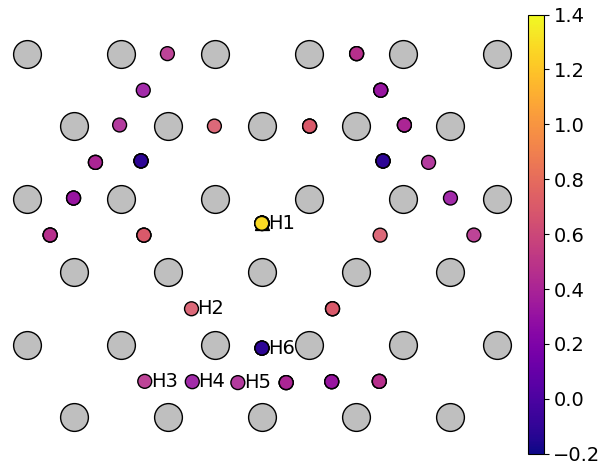
\includegraphics[width=0.85\textwidth]{../Images/hard_core_fe_C_positioning_energies.png}  \\

     	     \end{tabular}		
\caption{ Final positions and binding energies (eV) of carbon around the easy core (top) and hard core (bottom). The core was constrained by fixing the top and bottom three atoms surrounding each of the cores. As shown by Ventelon cite:Ventelon2015, the first and second closest octahedral sites to the hard core have their minimum energy inside the hard core. }
   \end{table}


Following the paper by Itakura
\cite{itakura13_effec_hydrog_atoms_screw_disloc} we calculated the
binding energy of carbon each of the screw dislocation cores. 

The solution energy is given by 
\[ E_s = E_{\text{d + C}} - E_{\text{d}} - E_{\text{C ref.}}, \]
where \(E_{\text{d + C}}\) is the total energy of a relaxed cluster with a
carbon interstitial and a dislocation, \(E_{\text{d}}\) is the total
energy of a relaxed cluster with a dislocation and \(E_{\text{C
    oct.}}\) is the total energy of relaxed a cluster with a single carbon in
an octahedral site.

The zero-point energy is calculated as in Itakura. After relaxation of the
C-dislocation system, a 3x3 Hessian matrix is constructed by taking the
numerical derivative of forces observed on the carbon atom after
displacement by \(\pm 0.015 \AA\) in each of the \(X\), \(Y\) and \(Z\) directions.
The three atoms surrounding the core on the first and third layers were
again fixed in \(Z\) coordinate. The zero-point energy is
given by

\[ E_z = \frac{1}{2} \sum_{i=1}^3 \frac{h}{2\pi} \sqrt{ k_i /
    m_{\text{C}} },  \]
where \(k_i\) are the eigenvalues of the Hessian and \(m_\text{C}\) is
the mass of carbon. 

The ZPE corrected solution energy is given by 
\[ E^{\text{Z}}_{s} = E_s + \Delta E_z,  \]

where \(\Delta E_z = E_z - E_{z\text{C ref.}}\) and \(E_{z\text{C ref.}} = 202.5 meV\) is the zero-point energy of carbon
situated in an octahedral site in a perfect cluster of the same size. 





\begin{table*}
\label{org1f8154f}
    \begin{tabular}{cccccc}
    \hline
Site Type & distance from core [b] & $E^{z}$ [eV] & $\Delta E^{z}$ [eV] & $E_b$ [eV] & $E_b^{z}$ [eV]  \\ 
     \hline
% 00        &                    --  &   0.203      &               0.000 &             &         --     \\
%           &                        &              &                     &             &                \\
E1        &                   0.57 &   0.185      & 	     -0.018 &       0.793 &          0.775 \\
E2        &                   0.70 &   0.202      & 	     -0.001 &       0.793 &          0.793 \\
E3        &                   0.99 &   0.205      & 	      0.002 &       0.137 &          0.139 \\
E4        &                   1.21 &   0.208      & 	      0.005 &       0.229 &          0.234 \\
E5        &                   1.36 &   0.210      & 	      0.008 &       0.784 &          0.791 \\
E6        &                   1.66 &   0.209      & 	      0.007 &       0.597 &          0.603 \\
E7        &                   1.89 &   0.206      & 	      0.003 &       0.385 &          0.388 \\
E8        &                   1.77 &   0.203      & 	      0.000 &       0.177 &          0.178 \\
H1        &                   0.00 &   0.196      & 	     -0.006 &       1.298 &          1.291 \\
H2        &                   1.19 &   0.210      & 	      0.007 &       0.691 &          0.698 \\
H3        &                   2.12 &   0.209      & 	      0.007 &       0.461 &          0.467 \\
H4        &                   1.91 &   0.207      & 	      0.005 &       0.311 &          0.316 \\
H5        &                   1.80 &   0.208      & 	      0.006 &       0.403 &          0.409 \\
H6        &                   1.40 &   0.207      & 	      0.005 &      -0.119 &         -0.114 \\

    \end{tabular}		
    \caption{Table of energies leading to the zero-point energy corrected binding energy. }
\end{table*}

These binding energies agree well with experiment and previous
calculations. The maximum binding energy found by the Fe-C EAM
potential by Becquart \cite{Becquart2007}, was 0.41eV. Kamber
\emph{et al.} found a maximum binding energy of 0.5 eV. Cochardt
found a value of 0.71 eV, which is within 0.1eV of the largest
binding energy for the easy core. 

EAM calculations by Clouet \cite{Clouet2008} found a binding energy of ---- by calculating the
elastic dipole tensor within Eshelby theory. 
Hanlumyuang \emph{et al.} \cite{Hanlumyuang2010} conducted DFT calculations for the interaction energy 12\AA{} from the core,
and their calculations agreed with the continuum limit of Eshelby theory with ----. 


In work by Ventelon \cite{Ventelon2015}, they found the interaction energy, in this convention of
an attractive energy being positive, as 0.79eV for a thickness in the \(Z\) direction of 3\(b\),
which is lower than the 1.29eV interaction energy of tight-binding. This indicates a reduction
in attraction in DFT calculations than in the tight-binding model. This discrepancy can be
partially explained due to the short cutoff of the carbon interactions in tight-binding---at
\(\sim a_{\text{bcc}} = 2.87 \AA\). As the carbon is separated from its periodic image by \(3b =
    8.61\AA\), there is no contribution from the repulsive C-C interaction from periodic images,
which is included within DFT.








Distance dependence of binding energies. 

\begin{center}
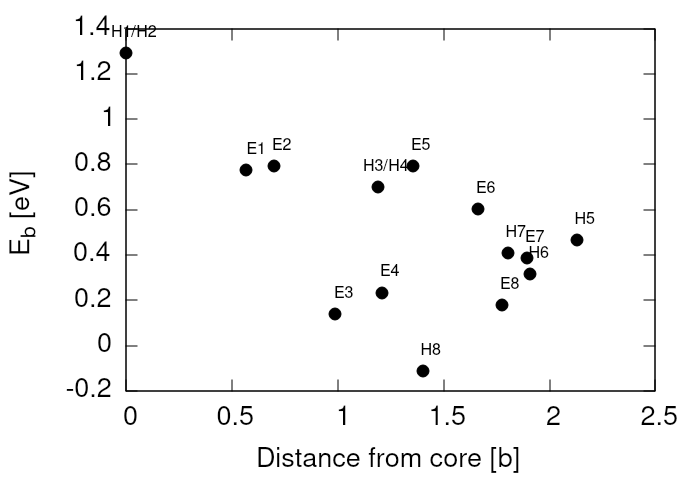
\includegraphics[width=.9\linewidth]{/home/tigany/Documents/docs/Management/Images/temp_binding_energy_distance_C_Fe.png}
\end{center}



\subsection{Line Tension}
\label{sec:org73d9443}


One is still doing the work for the line tension model. This model views the dislocation
as an elastic string which moves on the Peierls potential \(\Delta E_{\text{P}}\). One is
using the julia implementation of the NEB algorithm by Ortner \cite{Makri2019}.
The equilibrium line shape \(y(x)\) of the dislocation is the solution to the 1D Klein-Gordon
type equation \cite{Rodney2009}:

\[ - \frac{\text{d} ( \Delta E_{\text{P}}[y(x)] )}{\text{d} y(x) } + \sigma_{\text{A}} b + T \frac{\partial^2 y}{\partial x^2} = 0,\]

where, 

\[ T = E_L + \frac{\text{d}^2 E_L}{\text{d}\phi^2},  \]


\[ E_L = E_{\text{el}} + E_{\text{core}} = \frac{\mu b^2}{2\pi} \text{ln} \big
   ( \frac{R}{r_c}\big ) + E_{\text{core}}.\]


I have calculated the coefficients necessary for the line tension model. But there seem
to be differences between what Itakura states in his paper and the coefficients that are
measured in the Proville paper \cite{Rodney2009}. 

One thing I can do to check the coefficients are correct, is to fit to the the kink
shape from Luke's thesis to obtain the correct value for the line-tension \(T\).

\section{Discussion}
\label{sec:org789a33d}


\begin{itemize}
\item How do the results of this work feed into C migration with
dislocations?
\item How valid is the theory we have vs Fu \emph{et al}.
\item 
\end{itemize}

\section{Future work}
\label{sec:orgb6bef35}

\begin{itemize}
\item Validation of line-tension model by reproduction of the dislocation line shape from
Itakura 2012 \cite{Itakura2012}.
\item Compare tbe dislocation line shape with Itakura, and find the migration path of the dislocation from tbe data.
\item\relax [Optional] Find the elastic dipole tensor to check the binding energy of C within anisotropic elasticity.
\item Choose the sites for which one can fit a function (lorentzian) for the interaction energy between C and Fe.
\item Find the kink-pair formation enthalpy, with and without carbon, to feed into the kMC
code.
\end{itemize}

\section{Bibliography}
\label{sec:org8f4219d}
\label{org50b6242}

\bibliographystyle{unsrt}

\bibliography{../bibliography/org-refs}
\end{document}